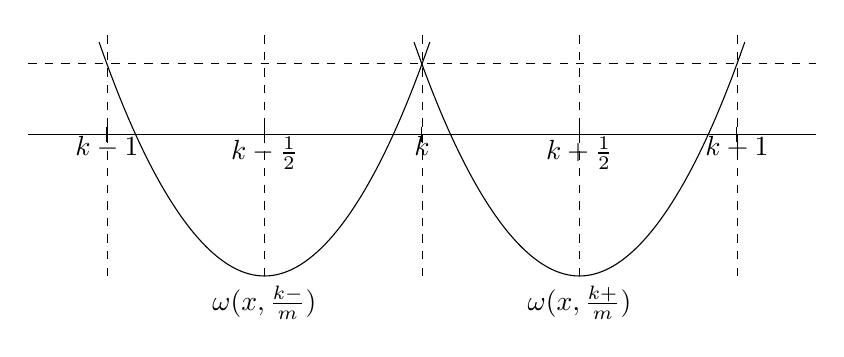
\begin{tikzpicture}[yscale=0.9]
  \draw (-5,0) -- (5,0);

  \foreach \x / \tick in {-4 / k-1, -2 / k-\frac{1}{2}, 0 / k, 2 / k+\frac{1}{2}, 4 / k+1}
  {
    \draw (\x cm,-3pt) -- (\x cm, 3pt) node[anchor=north] {$\tick$};
    \draw[very thin, dashed] (\x cm,-2cm) -- (\x cm,1.5cm);
  }
    
  \draw (-4.1,1.3) parabola bend (-2,-2) (0.1,1.3);
  \draw (-2,-2)node[anchor=north] {$\omega(x,\frac{k-\DCo}{m})$};
  
  
  \draw (-0.1,1.3) parabola bend (2,-2) (4.1,1.3);
  \draw (2,-2)node[anchor=north] {$\omega(x,\frac{k+\Co}{m})$};
  
  \draw[very thin,dashed] (-5,1) -- (5,1);
\end{tikzpicture}

%%% Local Variables:
%%% coding: cp1251
%%% mode: latex
%%% TeX-master: "../dissertation"
%%% End: